\chapter{Literature Review}\label{C:lit}

The analysis of complex time series has long relied on both time-domain and frequency-domain techniques. 
However, traditional methods often fall short in capturing nonlinear dynamics or are limited by strict assumptions such as stationarity and Gaussianity. 

The ordinal symbolic approach introduced by Bandt and Pompe in 2002 marked a significant theoretical advance by enabling robust, model-free characterization of time series. 
Their approach, rooted in information theory, involves converting segments of time series data into symbols based on the ordinal (rank) relationships among the data points.
These symbols are called "ordinal patterns." After computing all the symbols, their relative frequencies are used to estimate the probability distribution of ordinal patterns.

From this distribution estimate, two key descriptors entropy and complexity are calculated to characterize the time series: the scaled Shannon entropy, now widely known as permutation entropy, and the statistical complexity.

This chapter is divided into four main sections. Section~\ref{Sec:Onset} presents a brief overview of the area, focusing on what we consider the four seminal papers. Section~\ref{Sec:ResearchQuestion} discusses the research question and the motivation for conducting the bibliometric analysis. The final section, Section~\ref{Sec:BiblioIntro}, highlights the importance of bibliometric analysis and presents the results obtained from references that cite the Bandt and Pompe methodology and other related topics based on our research focus. 
Section~\ref{Sec:StatisitcalProperty} discusses the statistical properties of features from ordinal patterns based on the literature review.   
%\textcolor{red}{COMPLETE WITH ONE LINE}


\section{The Onset of the Entropy-Complexity Plane}\label{Sec:Onset}

This section discusses the emergence of the entropy-complexity plane. This topic is presented as a central theme because it reflects the foundation of our main research focus and illustrates how it has evolved over time into the current approach to time series analysis based on the concept of ordinal patterns. 

López-Ruiz et al.~\cite{lopez1995statistical} to capture the structure of a system:
the product between the entropy and a distance between the estimated model and a non-informative model is an interesting way of measuring complexity.
Lamberti et al.~\cite{lamberti2004intensive}, using that idea, proposed using the Euclidean distance between the measured probability function and the uniform distribution.
Rosso et al.~\cite{EEGAnalysisUsingWaveletBasedInformationTools} discussed using other distances, proposed the Jensen-Shannon distance, and used it jointly with the scaled Shannon entropy to form a bivariate feature.
They mapped this feature into the so-called ``Entropy-Complexity Plane,'' devising  a powerful diagnostic tool to distinguish between different dynamical regimes, such as chaos, noise, and periodicity.
Further, Martin et.al.~\cite{Martin2006} discussed the boundaries of this generalized statistical complexity measure. 

In the following, we present the research question and the motivation for continuing this research. 

\section{Research Question and Motivation}\label{Sec:ResearchQuestion}

The primary research question guiding this study is:
\begin{quote}
	\textit{How can confidence intervals for generalized entropy measures (Shannon, Tsallis, Rényi, Fisher information measure) and their associated complexity metrics be used to improve the robustness and discriminative power of time series clustering techniques?}
\end{quote}

We are motivated to conduct a literature review to confirm the relevance of our research areas in relation to the research question. Our aim is to determine whether other researchers are engaging with similar types of questions. Additionally, we seek to verify whether there is a strong focus on practical applications within this topic. 


\section{The Bibliometric Analysis: data collection, tools and background}\label{Sec:BiblioIntro}

Bibliometric analyses provide a quantitative approach to reviewing and mapping the intellectual structure of a research field. By systematically analyzing citation patterns, author collaborations, and keyword co-occurrences, they help identify key themes, research trends, and emerging topics. This method ensures objectivity, reveals key contributions, and offers a structured overview of intellectual development, making it a valuable tool for systematic literature reviews.

In this study, we conducted a bibliometric analysis using the Bibliometrix package in R and its user-friendly web interface Biblioshiny~\cite{Aria2017} focusing on literature related to ordinal patterns, permutation entropy, and complexity measures in time series analysis. 

Section~\ref{Subsec:Dataextraction} discusses the data extraction process using the Bibliometrix package in R.
%%% ACF Cite it

\subsection{Conceptual Structure: Data extraction and Summary Statistics}\label{Subsec:Dataextraction}

%%% ACF Make it clear that this is the data extraction phase
Scopus-indexed references that cited the seminal work by Bandt and Pompe, along with other references relevant to our research topic, were collected on June 9, 2025.
Based on these reference files, we analyzed a dataset consisting of 4125 reference files spanning the years 1993 to 2025. %%% ACF If you used papers that cited B&P, how can there be papers from 1993?
%%% ACF REVISE REMOVE REDUNDANT PARTS OR MOVE THEM TO WHERE THEY BELONG
%%% ACF USE \siunitx
The descriptive analysis of the dataset revealed a total of 4063 usable documents (out of 4125; the others had missing data and were removed), sourced from 1317 
%%% ACF What are they? publication sources refer to the outlets where research outputs (like journal articles, conference papers, books, etc.) are published. 
publication sources. 
The dataset shows an annual growth rate of \SI{18.15}{\percent}, %%% ACF??? indicates the percentage increase or decrease in the number of items within that dataset over a specific year. This metric helps researchers understand the trend of scholarly activity in a particular field, showing whether research output is expanding, contracting, or remaining stable. 
involving 7254 authors, 
123 single-authored documents, 
\SI{27.32}{\percent} international co-authorship, 
with an average of 4.28 co-authors per document. 
The author keywords totaled 7667, 
with an average document age of 5.7 years, %%% ACF???the mean age of all documents (e.g., articles, books) included in a study, typically measured in years from their publication date. It provides insights into the lifespan of research within a specific field or domain and can indicate how quickly research findings are disseminated and cited. A lower average age suggests a more rapidly evolving field, while a higher average age might indicate more established or mature research areas. 
and 22.6 citations per document. 

\subsection{Thematic Map Analysis}

Thematic map helps to understand the research direction and the relevant topics for the future studies. Therefore, we motivated to analyse it. The axes of the thematic map depicts the strength of their internal (density), which reflects inter-cluster growth, and external (connectivity) relevance or significance of the study in a particular area (centrality). 

Figure~\ref{fig:ThematicMap} illustrates the thematic map derived from author keywords.

\begin{figure}[H]
	\centering
	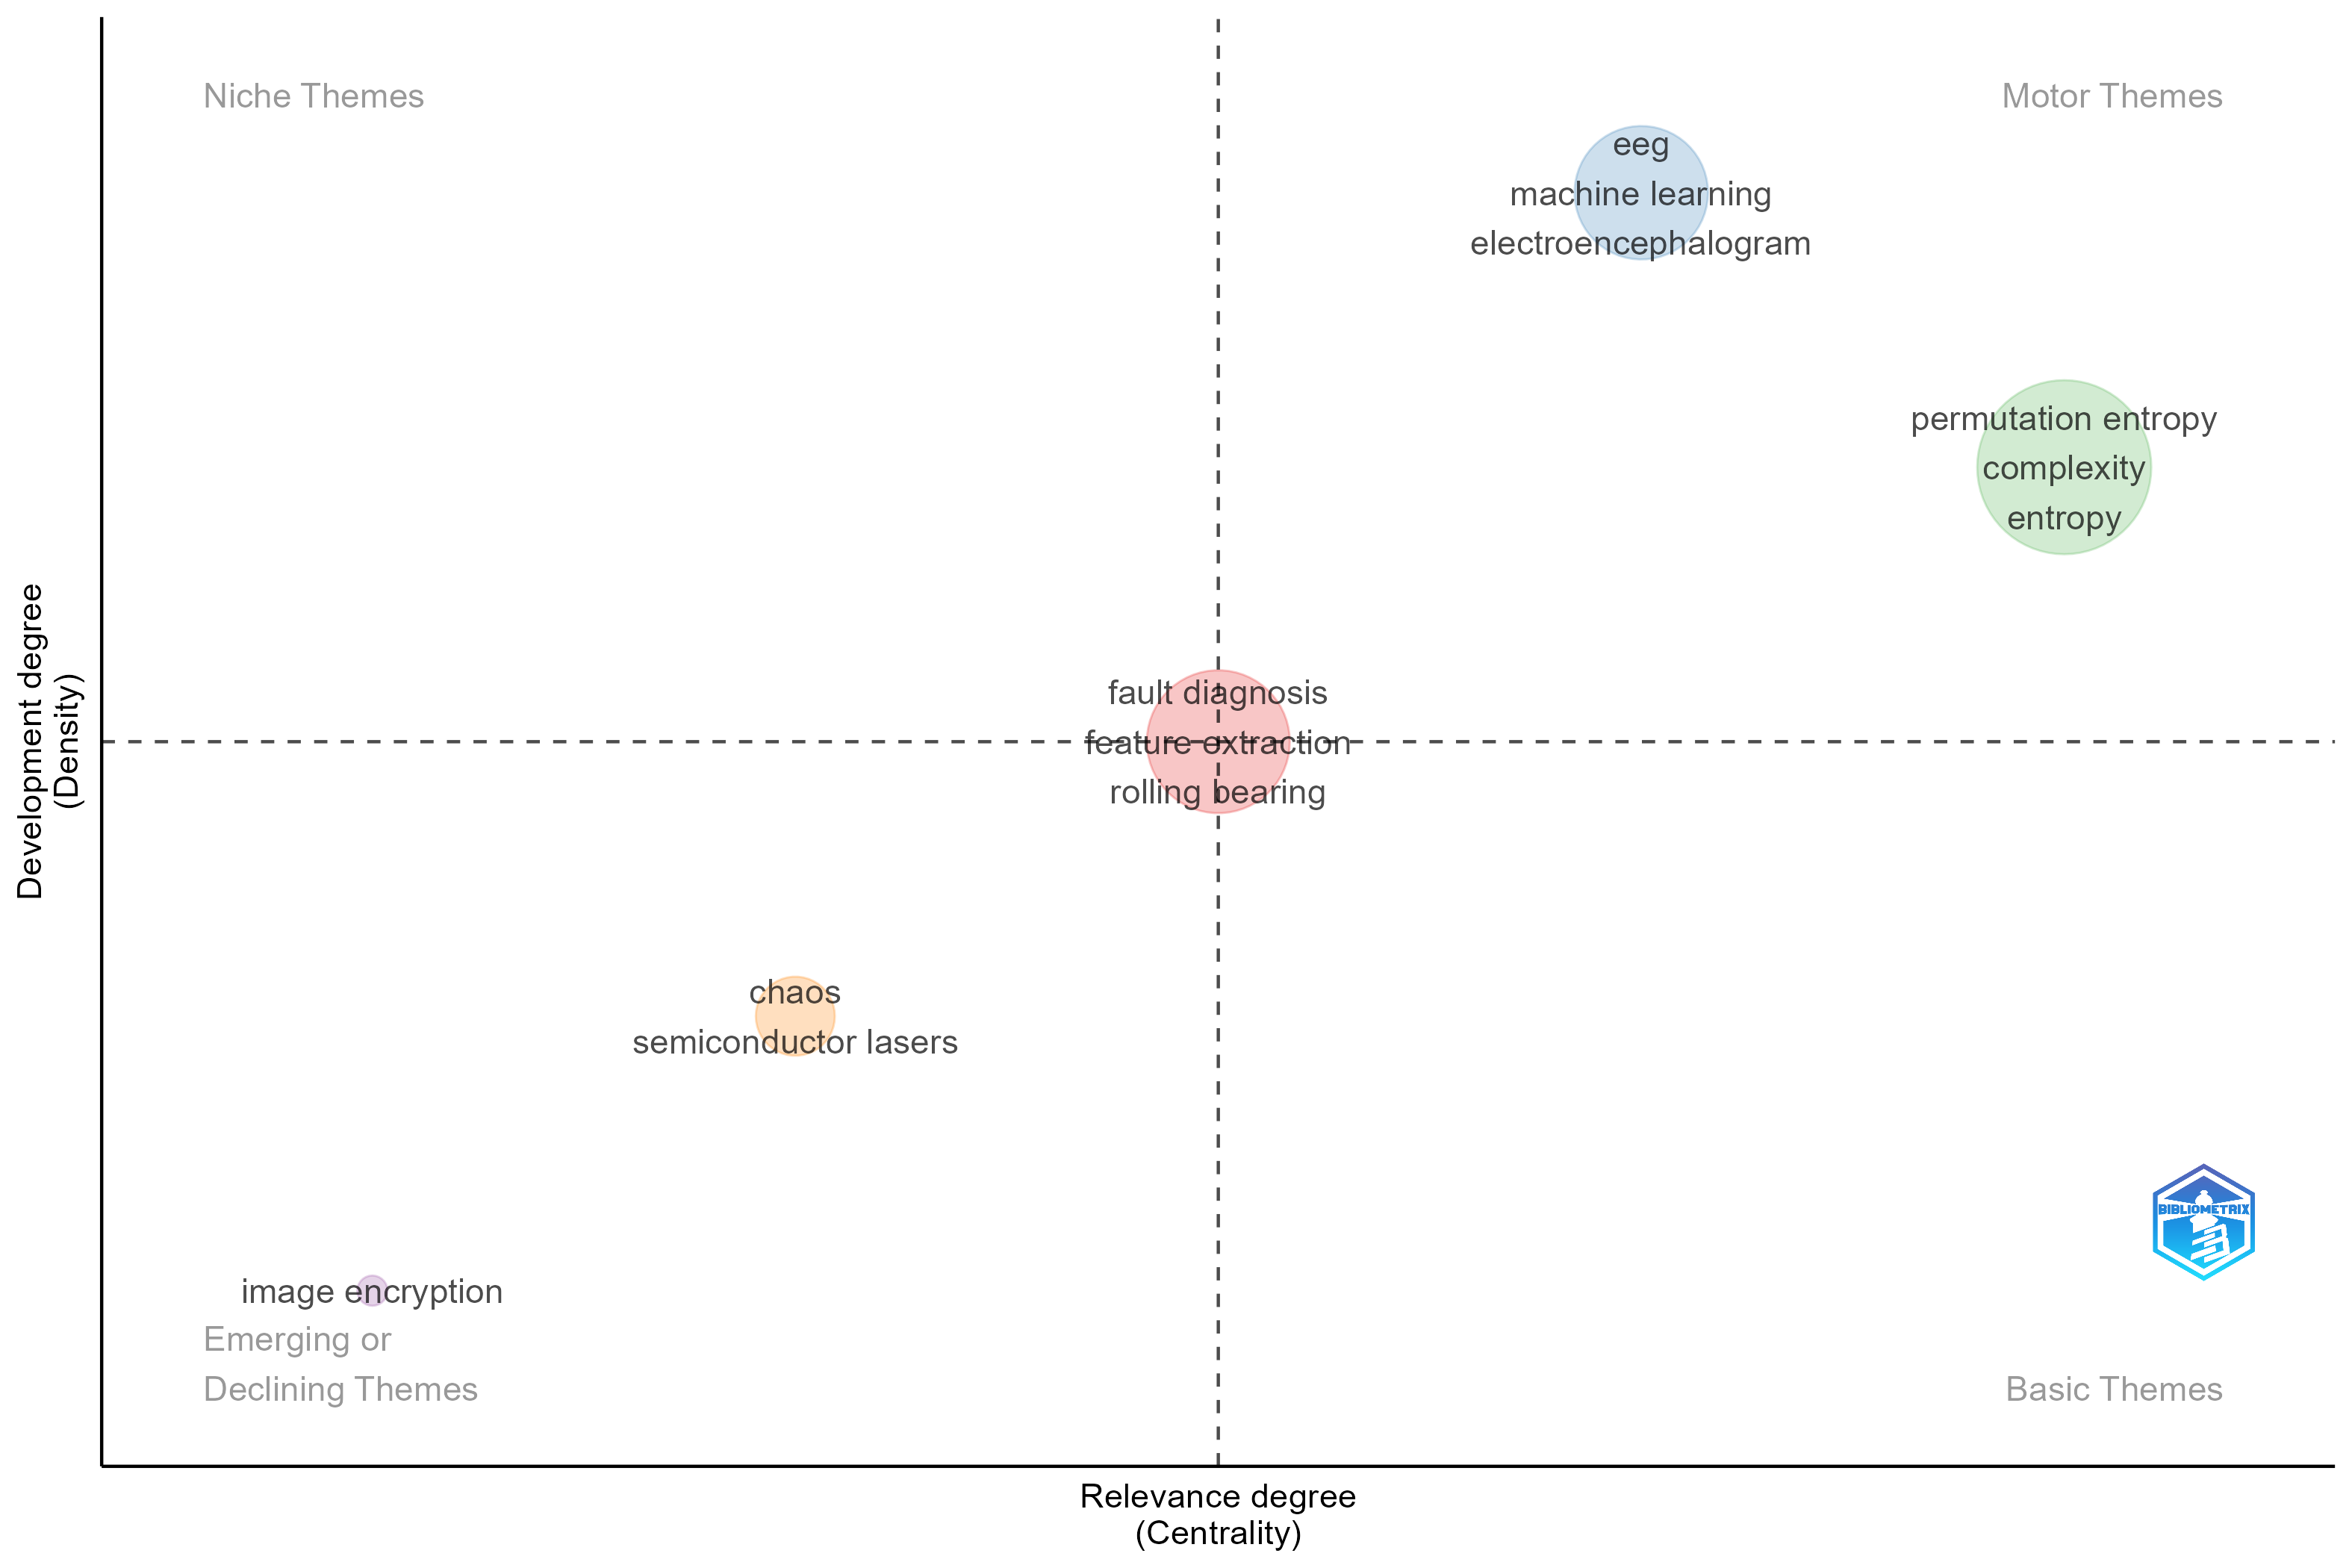
\includegraphics[width=\textwidth]{ThematicMap-2025-06-20}
	\caption{The Thematic Map generated by Bibliometrix.}
	\label{fig:ThematicMap}
\end{figure}

The map is divided into four quadrants based on two dimensions: centrality (relevance) and density (development). 
A right upper quadrant representing motor themes that are both well developed and highly interconnected areas of research, such as EEG, machine learning, permutation entropy, complexity, and other types of entropy. This theme is also at the core of current research, particularly in areas such as biomedical signal processing and nonlinear time series analysis. The consistent presence of entropy-based measures and machine learning highlights the interface between theory and practice.
%%% ACF What are Motor Themes? 

Emerging or declining themes like image encryption reflect peripheral or potentially declining research interests, while chaos and semiconductor lasers hold theoretical interest, but its practical integration appears limited.  

A right down quadrant depicts basic themes indicates that opportunities for further theoretical and methodological advancement. 
Research fields such as fault diagnosis, feature extraction and rolling bearings are at the center of the map. Its moderate centrality and density mean that it is still active and is subject to evolving research fields. These topics are closely linked to engineering and diagnostic applications. These are important and growing areas which require further methodological refinement and integration.
%%% ACF What are Basic Themes... and so on

The size of each circle further represents the frequency of the topic based on keyword occurrences associated with the publications. The clustering structure shows that entropy-related measures (such as the entropy of a permutation and the complexity of a system) are gaining ground not only in theory but also in practical applications such as EEG and machine learning.
%%% ACF This is NOT a thematic analysis. This is the output of bibliometrix. The thematic analysis starts from this evidence

From these results, we conclude that our research focus on entropy and complexity of permutation is relevant for many studies. These are basic concepts which are widely used in the literature, but which offer considerable potential for further development. Moreover, this thematic map shows that research is strongly focused on entropy-based methods, machine learning and biomedical applications, with fault diagnosis and feature extraction emerging as promising intermediate topics for further discuss.

%\textcolor{red}{From this results, we conclude that\dots}

\subsection{Factorial Analysis}
To identify the broad overview of the main research topics, we analyze the conceptual structure map. In this case we considered all keywords which are automatically generated by indexing databases. The shaded polygon in Figure~\ref{fig:factorialMap}  outlines the conceptual space defined by the most distinctive keywords. The X-axis (Dim 1) and the Y-axis (Dim 2) are the first two dimensions of the factorial space, and explain the largest differences in the co-occurrence of the keywords.

\begin{figure}[H]
	\centering
	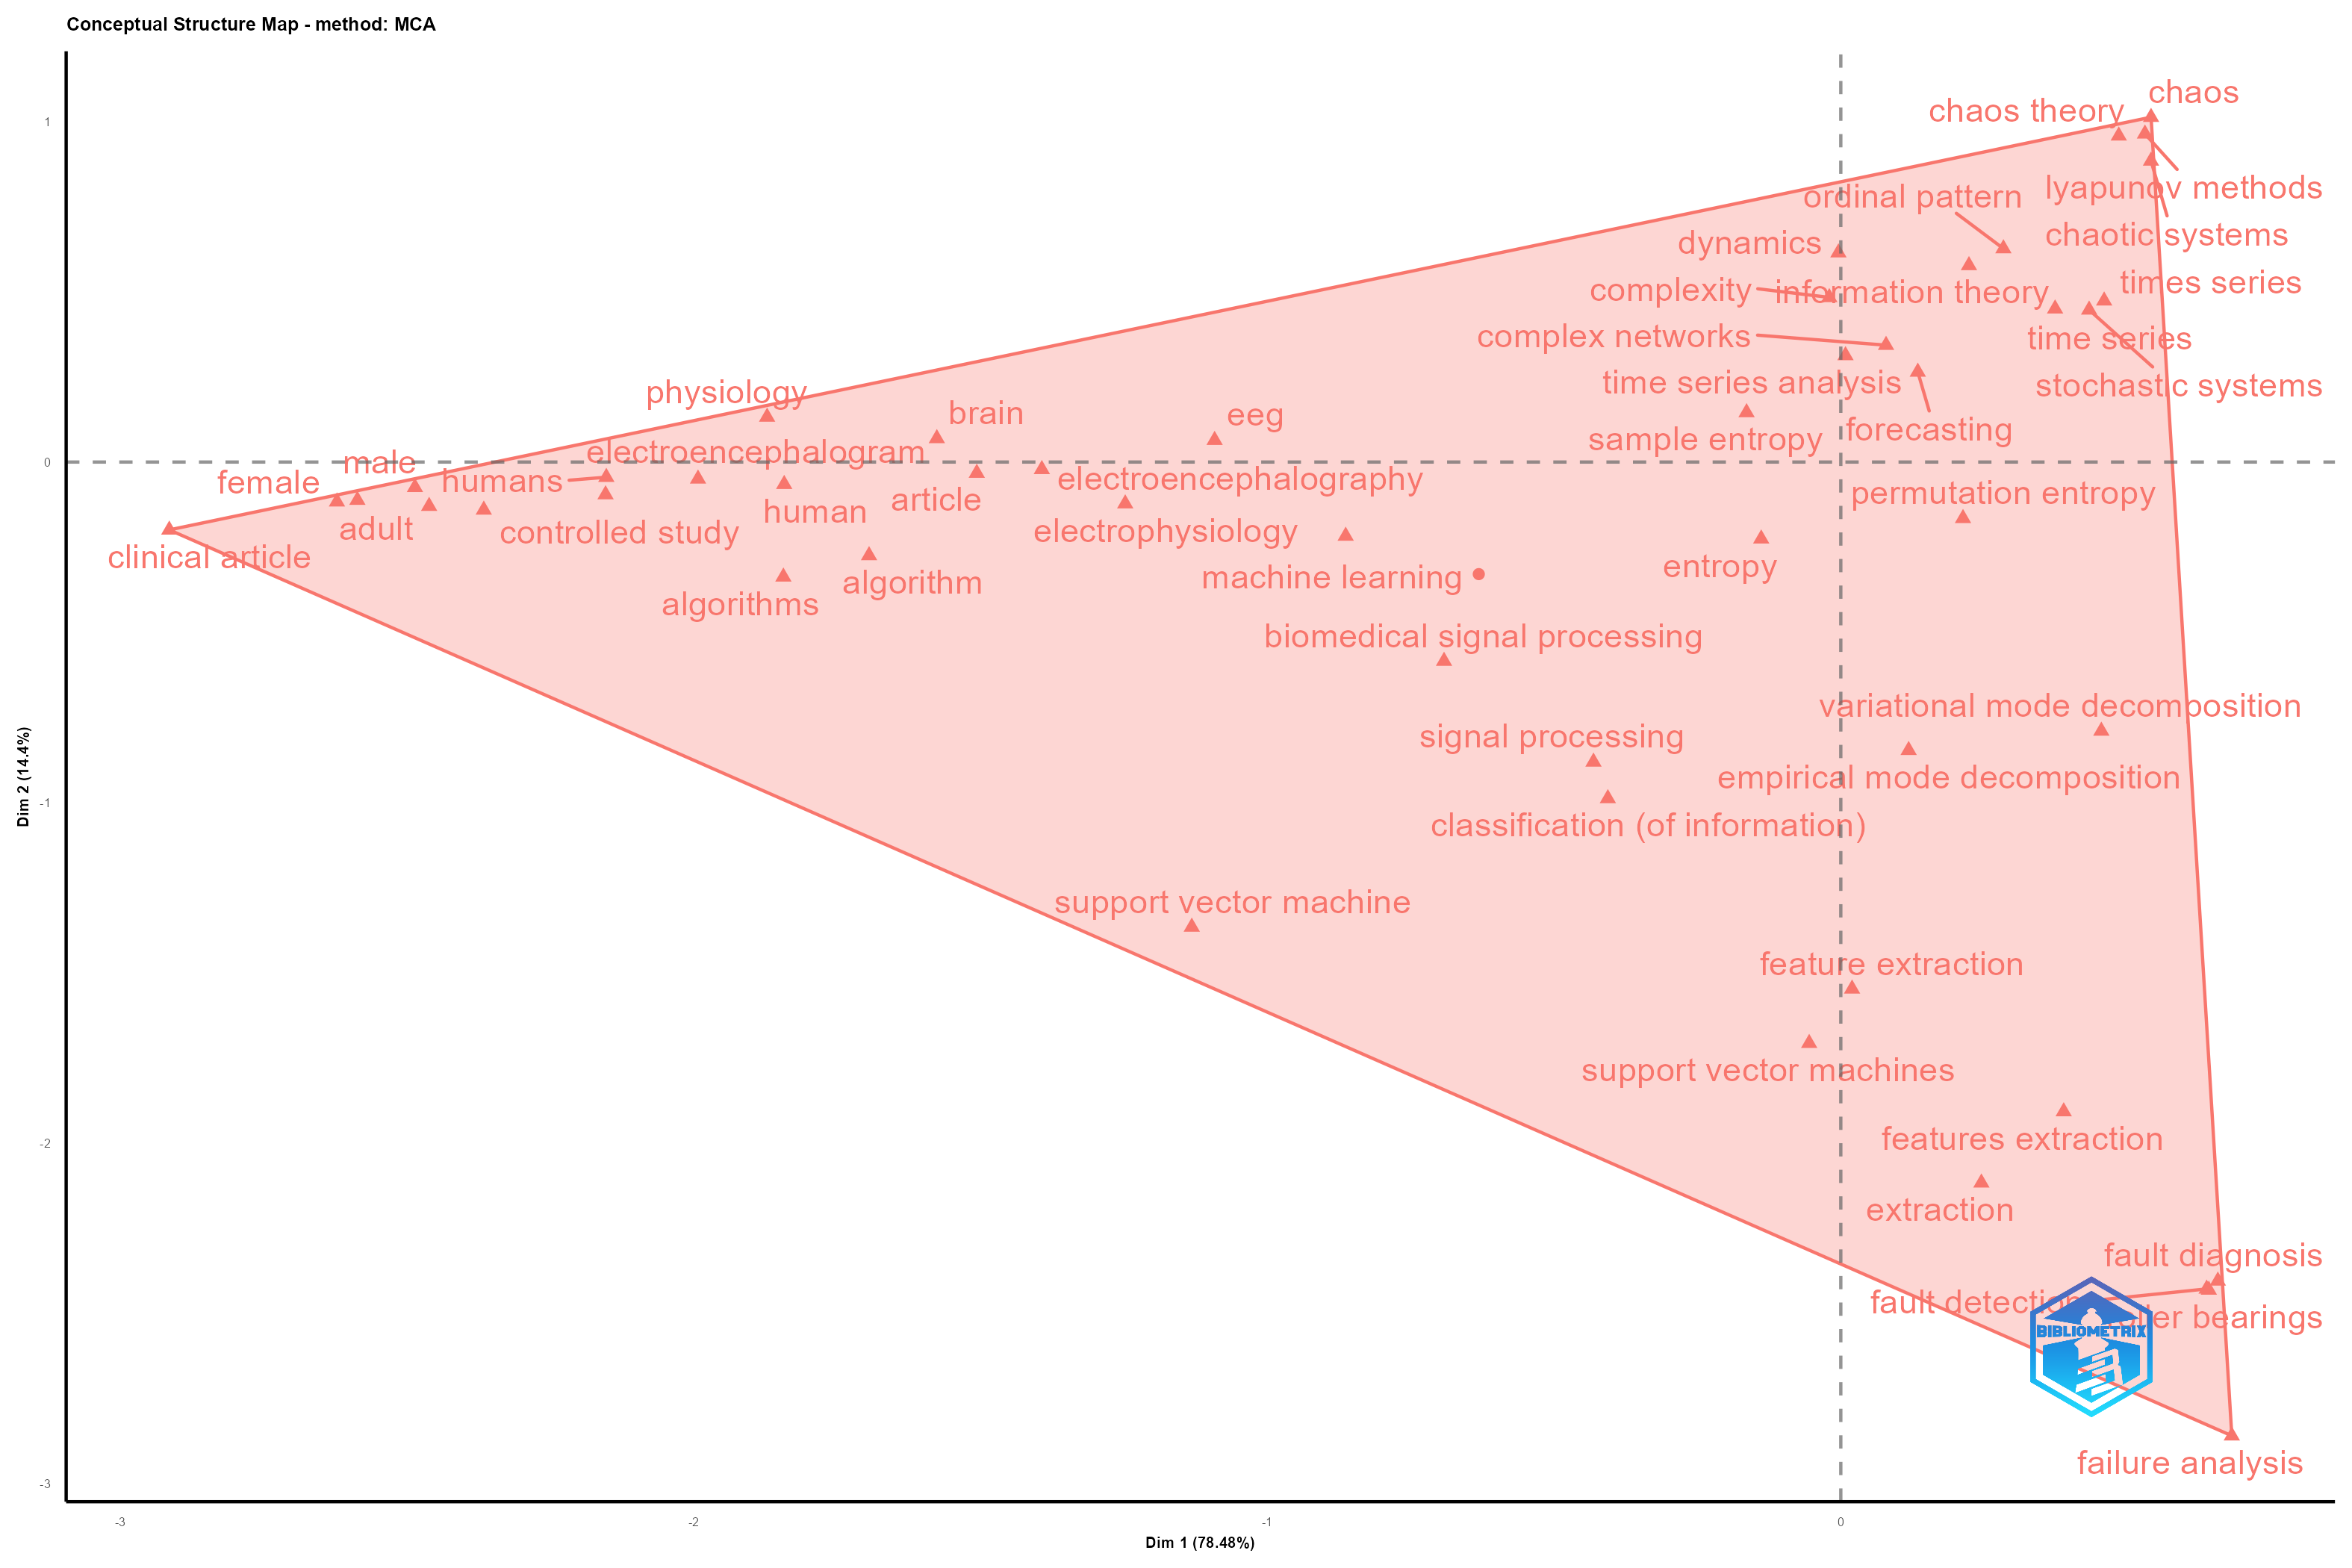
\includegraphics[width=0.9\textwidth]{FactorialMap}
	\caption{Conceptual Structure map generated by Bibliometrix.}
	\label{fig:factorialMap}
\end{figure}
%%% ACF Interpret: what do the axes mean? What does the point size encode?

The conceptual structure map reveals four major clusters:

The first cluster (upper right) includes theoretical concepts such as chaos theory, chaotic systems, Lyapunov methods, ordinal pattern, information theory, complex networks, and permutation entropy, forming the theoretical core of the research area.

The second cluster (lower right) includes practical applications such as feature extraction, empirical mode decomposition, variational mode decomposition, fault diagnosis, fault detection, and failure analysis, emphasizing the applied relevance of complexity-based time series analysis.

The third cluster (center) comprises terms related to biomedical signal processing and machine learning, including biomedical signal processing, EEG, support vector machine, classification, and machine learning, indicating the multidisciplinary applications of entropy measures.

A fourth, smaller cluster (left) includes clinical and physiological study keywords such as clinical article, controlled study, adult, male, female, humans, and physiology.

The conceptual map thus provides further evidence of the diverse applications and theoretical development surrounding ordinal patterns and complexity measures, supporting the originality and relevance of the present research.

%\textcolor{red}{MAKE YOUR CONCLUSIONS HERE. WHICH TOPICS AND WHY?}
\subsection{Conclusion and Justification of Research Focus}

Based on the thematic map and factorial analysis, research topics are categorized into four clusters and we will structure our review of the literature based on this clusters:

\begin{itemize}
	\item Permutation entropy, Complexity and other types of Entropy (section~\ref{Sec:ReviewTopicPE});
	\item EEG and Machine learning approach (section~\ref{Sec:ReviewTopicEEG});
	\item Fault diagnosis and failure analysis (section~\ref{Sec:ReviewTopicFault});
	\item Chaos other research works (section~\ref{Sec:ReviewTopicOthers});
	%\item Image encryption  (section~\ref{Sec:ReviewTopicImage}).
\end{itemize}

\section{Permutation entropy, Complexity and other types of Entropy}\label{Sec:ReviewTopicPE}
This cluster is associated with the keywords time series analysis, statistical complexity, nonlinear dynamics, ordinal patterns, entropy, and information theory. Although ordinal pattern based research have gained wide recognition as powerful tools for nonlinear time series analysis, with applications ranging from biomedical signal processing to cyber-physical systems, their theoretical and practical challenges remain unsolved \cite{Keller2017, Zanin2012}. 

Li et.al.~\cite{Li2015e} asses the complexity of short-term heartbeat interval series by using distribution entropy. They found that sample entropy (SampEn) or fuzzy entropy (FuzzyEn) quantifies essentially the randomness, which may not be uniformly identical to complexity. Zhang et.al.~\cite{Zhang2018d} uses the ordinal pattern technique to analyze dynamic behaviors such as regular, chaotic, or random patterns. The paper highlights the application of ordinal patterns in various fields, including ecology, finance, and physiology, where assessing variability and complexity is essential. It also emphasizes the advantages of using ordinal models to identify structural differences in time series that may not be detectable through traditional statistical methods.

Several studies have formalized the statistical behaviour of entropy and complexity measures derived from ordinal patterns, and have provided insights into their asymptotic distribution~\cite{Rey2024, Rey2023a} and sensitivity under the Multinomial law~\cite{Rey2023}. Despite these advances, the reliability of these measures in finite sampling conditions, in particular in non-stationary and noisy environments, remains limited~\cite{Borges2023}. 


Applications such as  Internet of Things(IoT) botnet detection~\cite{Borges2023} and  synthetic aperture radar(SAR) structure classification~\cite{Chagas2021a} have demonstrated the discriminability of ordinal-based features, particularly when combined with multiscale analysis; however, these methods often depend on the optimisation of parameters (dimension, delay) and may lack generalizability to a wide range of data. Similarly, the integration of entropy-complexity representations of class separation in time series dynamics~\cite{Borges2022}, although effective in a structured environment, poses problems when extended to real-time or data-scarce scenarios. 
%Data scarcity refers to the situation where there is insufficient data to meet the requirements of a system, particularly in enhancing the accuracy of predictive analytics.

The conceptual works linking ordinal complexity to broader ideas, such as the technological singularity~\cite{Modis2022} and the development of artistic expression ~\cite{Sigaki2018} illustrate the richness of the framework, but these studies are often qualitative and lack empirical rigour. 

Entropy-based clustering techniques have revealed evolving efficiency patterns in cryptocurrency markets~\cite{Sigaki2019}. The reliance on sensitive parameters and lack of standardized benchmarks highlight the need for more robust and interpretable methods to track market maturation reliably.

Moreover, white noise testing using entropy-complexity plane~\cite{Chagas2022a} and the use of ordinal properties in compressor signal diagnostics~\cite{Barbosa2024} demonstrate the methodological versatility of ordinal approaches. , the lack of uniform and reliable reference points prevents cross-domain comparison. Therefore, while ordinal methods provide a mathematically elegant and computationally efficient basis for obtaining information from complex signals, further research is needed to improve their statistical robustness, interpretability and adaptability to the challenges of the real world.

Although ordinal patterns are widely used in time series analysis, particularly in deriving entropy measures, studying their asymptotic distribution under the multinomial law, and analyzing the behavior of permutation entropy, their integration with confidence intervals remains widely unexplored. A systematic literature review reveals that while many studies investigate the statistical properties, asymptotic behavior, and robustness of ordinal pattern-based measures, no work has addressed the derivation or application of confidence intervals to assess the reliability or significance of time series clustering. This lack of statistical property limits interpretability and inference, especially when ordinal patterns are applied in data-driven algorithms. Therefore, this study aims to fill this gap by investigating how confidence intervals can be constructed for Shannon, Tsallis, and Renyi entropies, Fisher information measure, complexities, and how they may enhance time series clustering.
%%% ACF Do you need to describe again what the method is?
%Zanin et.al.~\cite{Zanin2012}  discuss the development and applications of permutation entropy, a method that captures the temporal structure and complexity of time series by analyzing the order relations among data points. 
%%% ACF Who is "He"?
%He focuses solely on probability distributions, permutation entropy incorporates temporal dynamics, making it particularly effective for studying chaotic and complex systems. 

\section{EEG and Machine learning approach}\label{Sec:ReviewTopicEEG}

%%% ACF Are EEG, epilepsy etc. "applications of entropy measures"?
This cluster is based on multidisciplinary studies involving entropy measures applied to areas such as EEG, epilepsy, classification, heart rate variability, deep learning methods, and nonlinear analysis. An analysis of the author keywords indicates that many of these studies are centered on applications in biomedical signal processing. 
%%% ACF Make the citation
Acharya et al. ~\cite{Acharya2015a, Acharya2015, Acharya2017, Acharya2016, Acharya2019,  Acharya2017a, Acharya2018} have made significant contributions to biomedical signal processing by developing and evaluating advanced automated diagnostic tools across a wide range of clinical applications. Their work includes the use of entropy measures to detect epilepsy and heart disease from EEG and ECG signals, as well as the use of nonlinear dynamics to enhance the detection of sleep stages and the characterisation of focal EEG signals. In the cardiovascular field, they have performed comparative studies on the localization of myocardial infarction using various ECG leads and have developed empirical decomposition methods to identify congestive heart failure from cardiac
%%% ACF Sort them so they appear in a sequence
signals. Another study by Lajnef et.al.~\cite{Lajnef2015} revealed that an automated approach to the classification of sleep stages using a multi-class support vector machine (SVM) based decision tree approach. The proposed method uses physiological signals (such as EEG, EOG, and EMG) to effectively classify the different stages of sleep.

\section{Fault diagnosis and failure analysis}\label{Sec:ReviewTopicFault}
This section primarily relates to the engineering applications of complexity-based time series analysis. The author keywords most commonly used to categorize this cluster include fault diagnosis, feature extraction, rolling bearing, support vector machine, variational mode decomposition, multiscale permutation entropy, dispersion entropy, rotating machinery, and empirical mode decomposition. 

Recent studies in bearing fault diagnosis often use entropy-based methods. Multiscale permutation entropy (MPE) and dispersion entropy are two popular techniques. These methods help detect complex changes in signals under different working conditions. For example, using variational mode decomposition with weighted entropy features helps extract useful information from non-stationary vibration signals. This improves how well faults can be classified~\cite{Lei2024a}. The weighted multiscale entropy method also works well by focusing on important frequency parts of the signal~\cite{Minhas2021a}. Self-adaptive hierarchical multiscale fuzzy entropy is also applied in bearing fault diagnosis. It makes fault detection easier without needing many manual settings~\cite{Yan2021}.  Composite multiscale fluctuation dispersion entropy can detect small fault signs even in noisy signals~\cite{Gan2019}. Some methods combine data decomposition with multiscale permutation entropy to better handle complex, changing systems~\cite{Yasir2018}. These improved entropy methods are also used in medical signal analysis, such as ECG or EEG, showing they work in other areas~\cite{Azami2017, HumeauHeurtier2015}. Dispersion entropy is known for being fast and good at finding small signal changes~\cite{Rostaghi2019,Rostaghi2016}, whereas multiscale permutation entropy still has issues. It can be affected by the length of the signal, noise, and it can be slow to compute~\cite{HumeauHeurtier2015, Zheng2014c}. Multiscale Permutation Entropy (MPE) with the Natural Visibility Graph (NVG) to enhance the fault diagnosis of rolling bearings by capturing both the dynamic complexity and structural features of time series method is proposed by Ma et.al.~\cite{Ma2025}. However, the method may still face limitations related to computational cost, parameter sensitivity, and the requirement for relatively long and noise-free signals to ensure reliable multiscale analysis.Therefore, more research is needed to make these methods faster, better with noise, and easier to use in different fault diagnosis tasks.

\section{Chaos and Other research works}\label{Sec:ReviewTopicOthers}
Research works related to chaos, semiconductor lasers, and image encryption are discussed in this category. 
A self-synchronous chaotic stream cipher, designed to resist active attacks and limit error propagation during image transmission, is a novel technique for image encryption.~\cite{Fan2018}. The 2D discrete wavelet transform, Arnold mapping, and a four-dimensional hyper-chaotic system with positive Lyapunov exponents are used to enhance the security and complexity of the encryption method. The advancement of chaos-based encryption and intelligent video security techniques in modern information systems has been demonstrated through a successful hardware implementation that transforms non-chaotic systems into chaotic ones, significantly enhancing unpredictability for secure communication. In addition, temporal action segmentation for video encryption has been analyzed to optimize computational resources and improve data protection~\cite{Gao2024,Liu2024k}
%\section{Image Encryption}\label{Sec:ReviewTopicImage}

\section{Statistical Properties of Features from Ordinal Patterns}\label{Sec:StatisitcalProperty}

Although ordinal pattern based methods, such as permutation entropy, have been widely used for nonlinear time series analysis, the statistical properties of the features derived from these patterns, such as their distribution, variance, and confidence intervals remain under-explored and require further theoretical and empirical investigation. Therefore, based on the literature review we investigate the researchers who worked related to ordinal patterns, what kind of statistical properties of features used for their research work. Table~\ref{tab:StatisticalProperties} provides more information about the research articles and the test statistics or distributions they used.


\begin{longtable}{|p{5.5cm}|p{2.5cm}|p{6.5cm}|}
	\caption{The test statistics used by the research articles for hypothesis testing}
	\label{tab:StatisticalProperties} \\
	\hline
	\textbf{Paper Title/Reference} & \textbf{Distribution} & \textbf{Brief Description} \\
	\hline
	\endfirsthead
	
	\multicolumn{3}{c}%
	{{\bfseries \tablename\ \thetable{} -- continued from previous page}} \\
	\hline
	\textbf{Paper Title/Reference} & \textbf{Distribution} & \textbf{Brief Description} \\
	\hline
	\endhead
	
	\hline \multicolumn{3}{r}{{Continued on next page}} \\
	\endfoot
	
	\hline
	\endlastfoot
	
	A non-parametric independence test using permutation entropy. Matilla-García et.al.~\cite{MatillaGarcia2008} & Empirical (permutation) distribution & Tests independence by comparing the observed permutation entropy-based statistic to its distribution under random shuffling (permutation) of the time series.\\
	\hline
	Asymptotic distribution of certain types of entropy under the multinomial law. Rey at.at.~\cite{Rey2023} & Normal, Chi-squared ($\chi^2$) & Analyzes the asymptotic distribution (normal and chi-squared) of entropy estimators under the multinomial law. \\
	\hline
	Asymptotic distribution of entropies and Fisher information measure of ordinal patterns with applications. Reyet.al.~\cite{Rey2024} & Normal, Chi-squared ($\chi^2$) & Provides asymptotic distributions for entropy and Fisher information measures of ordinal patterns. \\
	\hline
	Asymptotic distribution of the permutation entropy. Rey at.al.~\cite{Rey2023a} & Normal & Derives the asymptotic normal distribution for permutation entropy estimators. \\
	\hline
	Asymptotic distribution of the statistical complexity under the multinomial law. Rey at.al.~\cite{Rey2025} & Normal, Chi-squared ($\chi^2$) & Studies the asymptotic distribution of statistical complexity measures derived from ordinal patterns under the multinomial law. \\
	\hline
	Assessing serial dependence in ordinal patterns processes using chi-squared tests with application to EEG data. Yamashita et.al.~\cite{YamashitaRiosDeSousa2022} & Chi-squared ($\chi^2$) & Applies chi-squared tests to assess serial dependence in ordinal pattern processes, with application to EEG data. \\
	\hline
	Bearing fault diagnosis based on Alpha-stable distribution feature extraction and SVM classifier. Chouri et.al.~\cite{Chouri2014} & Alpha-stable & Uses alpha-stable distribution parameters for feature extraction and SVM for classification in bearing fault diagnosis. \\
	\hline
	Belief permutation entropy of time series: A natural transition in analytical framework from probability theory to evidence theory. Xie et. al.~\cite{Xie2025} & Belief functions, Evidence theory basis & Introduces belief permutation entropy (BPE) using evidence theory (belief functions and mass assignments) and Deng entropy instead of classical probability distributions. \\
	\hline
	Markov modeling via ordinal partitions: An alternative paradigm for network-based time-series analysis. Sakellariou et.al.~\cite{Sakellariou2019} & Markov (transition) probabilities & Uses Markov models constructed from ordinal partitions to analyze time series as networks. \\
	\hline
	On the statistical properties of Multiscale Permutation Entropy: Characterization of the estimator's variance. Dávalos et.al.~\cite{Davalos2019a} & Normal (asymptotic) & Shows that the multiscale permutation entropy estimator is asymptotically normally distributed, allowing inference on variance.\\
	\hline
	Price predictability at ultra high frequency:Entropy based randomness test. Shternshis et.al.~\cite{Shternshis2025}& Chi-squared ($\chi^2$) & Proposes a randomness test for time series based on entropy, with asymptotic chi-squared distribution for the test statistic. \\
	\hline
	Statistical properties of the entropy from ordinal patterns. Chagas et.al.~\cite{Chagas2022} & Normal & Investigates statistical properties and asymptotic normality of entropy estimators from ordinal patterns. \\
	\hline
	The asymptotic distribution of the permutation entropy. Rey at.al.~\cite{Rey2023a} & Normal & Derives the asymptotic normal distribution for permutation entropy estimators. \\
	\hline
	The modified permutation entropy-based independence test of time series. Ashtari et.al.~\cite{AshtariNezhad2019} & Empirical (permutation) distribution & Tests independence by comparing the observed permutation entropy-based statistic to its distribution under random shuffling (permutation) of the time series.\\
	\hline
	White Noise Test from ordinal patterns in the entropy-complexity plane. Chagas et.al.~\cite{Chagas2022a} & Empirical Distribution & Used in white noise tests by repeatedly shuffling the time series to estimate the null distribution of the test statistic.\\
	\hline
	 Variance of entropy for testing time-varying regimes with an application to meme stocks Shternshis et.al.~\cite{Shternshis2024} & Chi-squared ($\chi^2$) & Introduces a rigorous hypothesis testing framework featuring an unbiased analytic approximation of sample Shannon entropy’s variance and an optimal rolling-window selection method.\\
	\hline
	
\end{longtable}









